\textcolor{lila}{Här presenteras huvuddragen av varje problem samt den tillhörande informationen. Notera att allt runtomkring själva problemet enbart är förslag, och att varje lärare kan anpassa genomförandet efter hur hen tror att det blir bäst i en specifik klass. Alla problemen finns även i sin fullständiga form i appendix~\ref{appendix:Problem}.}

\subsubsection{Fermiproblem}
    \label{sec:Fermi}
 
    \textcolor{lila}{Målet med detta problem är att eleverna ska få träna på att göra uppskattningar, samt att bryta ner ett problem i mindre delar.}
    
    \textcolor{lila}{Som inledning presenteras vad ett \textsl{fermiproblem} är. Det innebär att man, i fall där ett specifikt värde inte är svårt alternativt omöjligt att mäta, bryter ner problemet i många små delar och uppskattar varje del för sig. På så sätt kan man uppskatta lösningen på frågor som vid första anblick kan verka omöjliga. För att illustrera detta visas även ett exempel på ett fermiproblem, samt exempel på hur man kan dela upp det i minde delar.}

    \textcolor{lila}{Eleverna får en lista med olika fermiproblem att välja mellan, och ska arbeta i grupper om 2. Först ska de gissa på svaret, och sedan beräkna det genom att dela upp i delar som man kan uppskatta. Därefter får de i mindre grupper presentera och diskutera sitt arbete. Slutligen diskuteras i helklass om resultaten kändes rimliga, hur genomförandet gick, ifall lösningsmetoden är användbar samt varför den fungerar så bra som den gör. För den sista frågan ger vi även lärararen svaret, det vill säga att det fungerar eftersom man ibland överskattar och ibland underskattar de mindre delarna, vilket gör att det slutgiltiga resultatet ofta blir en mycket bra uppskattning.}

\subsubsection{Flygplan}
    \label{sec:Flygplan}
    
    \textcolor{lila}{Detta  problem syftar till att träna eleverna på ett undersökande arbetssätt där inte alla påverkande faktorer är givna, utan måste resoneras fram av eleverna. Den leder också fram till ett ekvationssystem, vilket ger ett exempel på när dessa är användbara.}
    
    \begin{figure}%[H]
        \centering
        %\hspace{-40pt}
        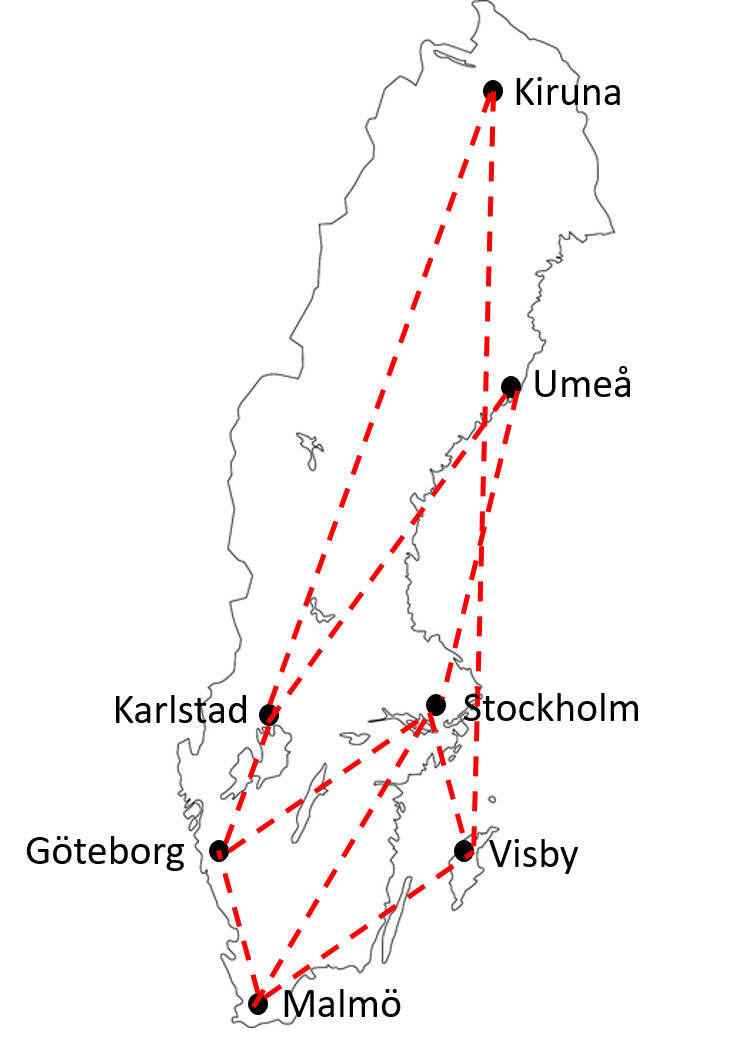
\includegraphics[width=0.4\textwidth]{Figures/Flygplan_rapport.png}
        \caption{\textsl{Den sverigekarta med utmarkerade flygplatser och rutter som presenteras för eleverna i uppgiften ''Flygplan''.}}
        \label{fig:Flygplan}
    \end{figure}
    
    \textcolor{lila}{En Sverigekarta med utmarkerade flygplatser och flygrutter presenteras för klassen, se figur~\ref{fig:Flygplan}. Detta görs bitvis, med plats för en kort diskussion om vad frågeställningen skulle kunna vara, givet den dittills givna informationen. Med all information given får eleverna i grupper om två arbeta med en specifik sträcka, Visby-Karlstad. På vilka olika sätt kan man ta sig mellan dessa två städer? Vilken sträcka är bäst och vilka faktorer påverkar detta? Därefter specificeras uppgiften ytterligare, genom att de får reda på hur mycket det kostar att åka mellan två olika dirketa flygsträckor. De ska nu hitta den \textsl{billigaste} vägen mellan Karlstad och Visby, samt vilken väg som blir billigast om man ska från Karlstad till Stockholm, men sträckan Stockholm-Göteborg är fullbokad. Den avslutande helklassdiskussionen tar bland annat upp vilka faktorer som påverkar bränslekostnaden, vilka faktorer som påverkar biljettpris för en specifik sträcka och ifall det är det totala avståndet eller antalet mellanlandningar som avgör priset för en resa.}
    
    \textcolor{lila}{Under punkten ''Ytterligare information'' diskuteras }
    
\subsubsection{Sortera en kortlek}
    \label{sec:Sortera}
    
    \textcolor{WildStrawberry}{
        Kortleken är ett enkelt sätt för en elev att få en god introduktion till hur enkla sorteringsalgoritmer fungerar samt hur man nyttjar sig av dem. }
        
    \textcolor{WildStrawberry}{
        Lektionen kommer innefatta att eleven får en beskrivning fundera en stund på vad}